\documentclass[1p]{elsarticle_modified}
%\bibliographystyle{elsarticle-num}

%\usepackage[colorlinks]{hyperref}
%\usepackage{abbrmath_seonhwa} %\Abb, \Ascr, \Acal ,\Abf, \Afrak
\usepackage{amsfonts}
\usepackage{amssymb}
\usepackage{amsmath}
\usepackage{amsthm}
\usepackage{scalefnt}
\usepackage{amsbsy}
\usepackage{kotex}
\usepackage{caption}
\usepackage{subfig}
\usepackage{color}
\usepackage{graphicx}
\usepackage{xcolor} %% white, black, red, green, blue, cyan, magenta, yellow
\usepackage{float}
\usepackage{setspace}
\usepackage{hyperref}

\usepackage{tikz}
\usetikzlibrary{arrows}

\usepackage{multirow}
\usepackage{array} % fixed length table
\usepackage{hhline}

%%%%%%%%%%%%%%%%%%%%%
\makeatletter
\renewcommand*\env@matrix[1][\arraystretch]{%
	\edef\arraystretch{#1}%
	\hskip -\arraycolsep
	\let\@ifnextchar\new@ifnextchar
	\array{*\c@MaxMatrixCols c}}
\makeatother %https://tex.stackexchange.com/questions/14071/how-can-i-increase-the-line-spacing-in-a-matrix
%%%%%%%%%%%%%%%

\usepackage[normalem]{ulem}

\newcommand{\msout}[1]{\ifmmode\text{\sout{\ensuremath{#1}}}\else\sout{#1}\fi}
%SOURCE: \msout is \stkout macro in https://tex.stackexchange.com/questions/20609/strikeout-in-math-mode

\newcommand{\cancel}[1]{
	\ifmmode
	{\color{red}\msout{#1}}
	\else
	{\color{red}\sout{#1}}
	\fi
}

\newcommand{\add}[1]{
	{\color{blue}\uwave{#1}}
}

\newcommand{\replace}[2]{
	\ifmmode
	{\color{red}\msout{#1}}{\color{blue}\uwave{#2}}
	\else
	{\color{red}\sout{#1}}{\color{blue}\uwave{#2}}
	\fi
}

\newcommand{\Sol}{\mathcal{S}} %segment
\newcommand{\D}{D} %diagram
\newcommand{\A}{\mathcal{A}} %arc


%%%%%%%%%%%%%%%%%%%%%%%%%%%%%5 test

\def\sl{\operatorname{\textup{SL}}(2,\Cbb)}
\def\psl{\operatorname{\textup{PSL}}(2,\Cbb)}
\def\quan{\mkern 1mu \triangleright \mkern 1mu}

\theoremstyle{definition}
\newtheorem{thm}{Theorem}[section]
\newtheorem{prop}[thm]{Proposition}
\newtheorem{lem}[thm]{Lemma}
\newtheorem{ques}[thm]{Question}
\newtheorem{cor}[thm]{Corollary}
\newtheorem{defn}[thm]{Definition}
\newtheorem{exam}[thm]{Example}
\newtheorem{rmk}[thm]{Remark}
\newtheorem{alg}[thm]{Algorithm}

\newcommand{\I}{\sqrt{-1}}
\begin{document}

%\begin{frontmatter}
%
%\title{Boundary parabolic representations of knots up to 8 crossings}
%
%%% Group authors per affiliation:
%\author{Yunhi Cho} 
%\address{Department of Mathematics, University of Seoul, Seoul, Korea}
%\ead{yhcho@uos.ac.kr}
%
%
%\author{Seonhwa Kim} %\fnref{s_kim}}
%\address{Center for Geometry and Physics, Institute for Basic Science, Pohang, 37673, Korea}
%\ead{ryeona17@ibs.re.kr}
%
%\author{Hyuk Kim}
%\address{Department of Mathematical Sciences, Seoul National University, Seoul 08826, Korea}
%\ead{hyukkim@snu.ac.kr}
%
%\author{Seokbeom Yoon}
%\address{Department of Mathematical Sciences, Seoul National University, Seoul, 08826,  Korea}
%\ead{sbyoon15@snu.ac.kr}
%
%\begin{abstract}
%We find all boundary parabolic representation of knots up to 8 crossings.
%
%\end{abstract}
%\begin{keyword}
%    \MSC[2010] 57M25 
%\end{keyword}
%
%\end{frontmatter}

%\linenumbers
%\tableofcontents
%
\newcommand\colored[1]{\textcolor{white}{\rule[-0.35ex]{0.8em}{1.4ex}}\kern-0.8em\color{red} #1}%
%\newcommand\colored[1]{\textcolor{white}{ #1}\kern-2.17ex	\textcolor{white}{ #1}\kern-1.81ex	\textcolor{white}{ #1}\kern-2.15ex\color{red}#1	}

{\Large $\underline{12n_{0112}~(K12n_{0112})}$}

\setlength{\tabcolsep}{10pt}
\renewcommand{\arraystretch}{1.6}
\vspace{1cm}\begin{tabular}{m{100pt}>{\centering\arraybackslash}m{274pt}}
\multirow{5}{120pt}{
	\centering
	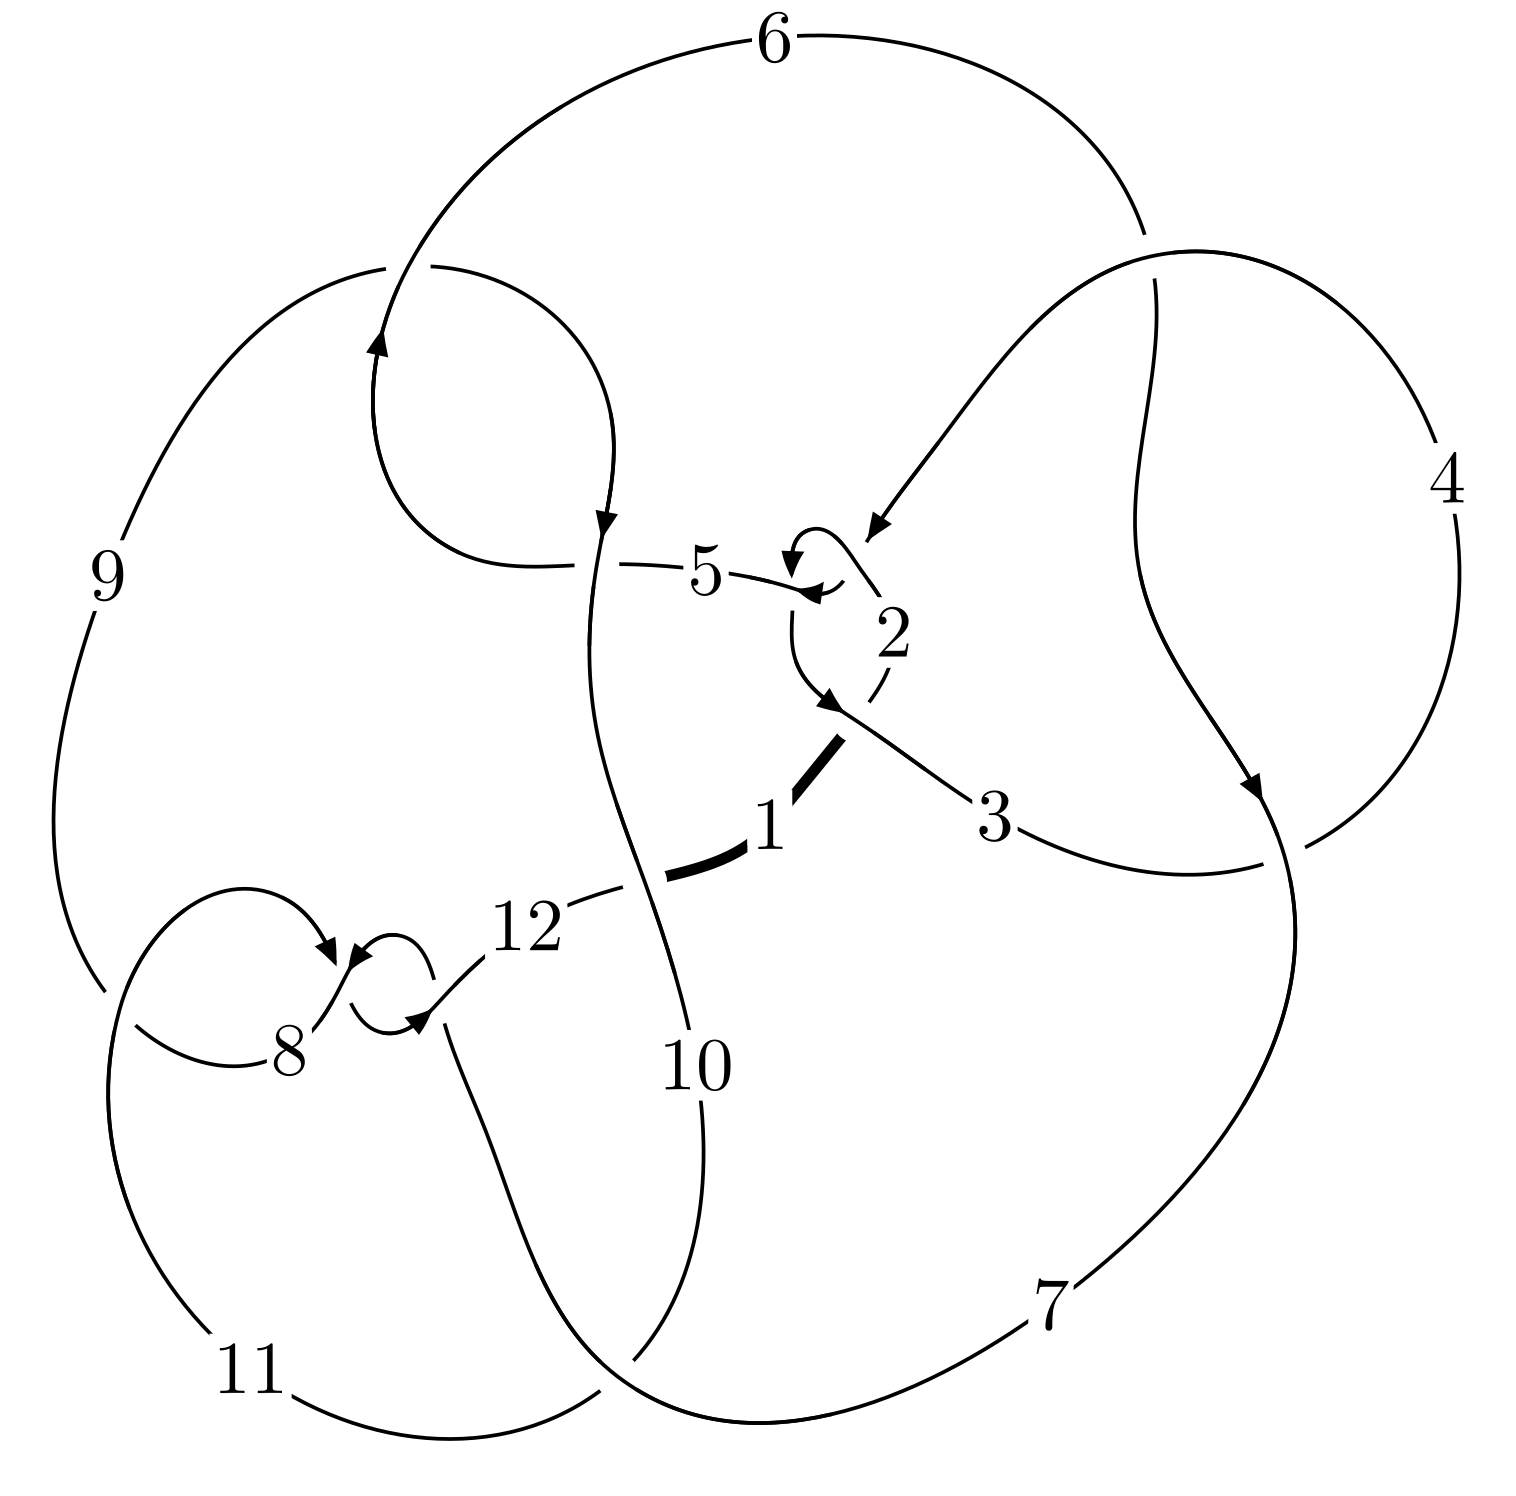
\includegraphics[width=112pt]{../../../GIT/diagram.site/Diagrams/png/2201_12n_0112.png}\\
\ \ \ A knot diagram\footnotemark}&
\allowdisplaybreaks
\textbf{Linearized knot diagam} \\
\cline{2-2}
 &
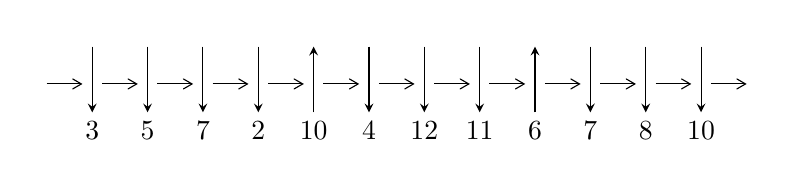
\begin{tikzpicture}[x=20pt, y=17pt]
	% nodes
	\node (C0) at (0, 0) {};
	\node (C1) at (1, 0) {};
	\node (C1U) at (1, +1) {};
	\node (C1D) at (1, -1) {3};

	\node (C2) at (2, 0) {};
	\node (C2U) at (2, +1) {};
	\node (C2D) at (2, -1) {5};

	\node (C3) at (3, 0) {};
	\node (C3U) at (3, +1) {};
	\node (C3D) at (3, -1) {7};

	\node (C4) at (4, 0) {};
	\node (C4U) at (4, +1) {};
	\node (C4D) at (4, -1) {2};

	\node (C5) at (5, 0) {};
	\node (C5U) at (5, +1) {};
	\node (C5D) at (5, -1) {10};

	\node (C6) at (6, 0) {};
	\node (C6U) at (6, +1) {};
	\node (C6D) at (6, -1) {4};

	\node (C7) at (7, 0) {};
	\node (C7U) at (7, +1) {};
	\node (C7D) at (7, -1) {12};

	\node (C8) at (8, 0) {};
	\node (C8U) at (8, +1) {};
	\node (C8D) at (8, -1) {11};

	\node (C9) at (9, 0) {};
	\node (C9U) at (9, +1) {};
	\node (C9D) at (9, -1) {6};

	\node (C10) at (10, 0) {};
	\node (C10U) at (10, +1) {};
	\node (C10D) at (10, -1) {7};

	\node (C11) at (11, 0) {};
	\node (C11U) at (11, +1) {};
	\node (C11D) at (11, -1) {8};

	\node (C12) at (12, 0) {};
	\node (C12U) at (12, +1) {};
	\node (C12D) at (12, -1) {10};
	\node (C13) at (13, 0) {};

	% arrows
	\draw[->,>={angle 60}]
	(C0) edge (C1) (C1) edge (C2) (C2) edge (C3) (C3) edge (C4) (C4) edge (C5) (C5) edge (C6) (C6) edge (C7) (C7) edge (C8) (C8) edge (C9) (C9) edge (C10) (C10) edge (C11) (C11) edge (C12) (C12) edge (C13) ;	\draw[->,>=stealth]
	(C1U) edge (C1D) (C2U) edge (C2D) (C3U) edge (C3D) (C4U) edge (C4D) (C5D) edge (C5U) (C6U) edge (C6D) (C7U) edge (C7D) (C8U) edge (C8D) (C9D) edge (C9U) (C10U) edge (C10D) (C11U) edge (C11D) (C12U) edge (C12D) ;
	\end{tikzpicture} \\
\hhline{~~} \\& 
\textbf{Solving Sequence} \\ \cline{2-2} 
 &
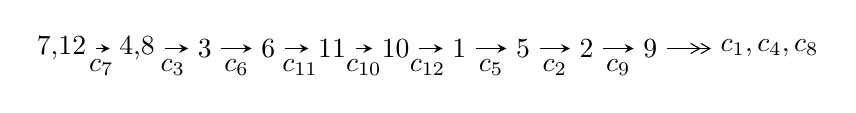
\begin{tikzpicture}[x=23pt, y=7pt]
	% node
	\node (A0) at (-1/8, 0) {7,12};
	\node (A1) at (17/16, 0) {4,8};
	\node (A2) at (17/8, 0) {3};
	\node (A3) at (25/8, 0) {6};
	\node (A4) at (33/8, 0) {11};
	\node (A5) at (41/8, 0) {10};
	\node (A6) at (49/8, 0) {1};
	\node (A7) at (57/8, 0) {5};
	\node (A8) at (65/8, 0) {2};
	\node (A9) at (73/8, 0) {9};
	\node (C1) at (1/2, -1) {$c_{7}$};
	\node (C2) at (13/8, -1) {$c_{3}$};
	\node (C3) at (21/8, -1) {$c_{6}$};
	\node (C4) at (29/8, -1) {$c_{11}$};
	\node (C5) at (37/8, -1) {$c_{10}$};
	\node (C6) at (45/8, -1) {$c_{12}$};
	\node (C7) at (53/8, -1) {$c_{5}$};
	\node (C8) at (61/8, -1) {$c_{2}$};
	\node (C9) at (69/8, -1) {$c_{9}$};
	\node (A10) at (11, 0) {$c_{1},c_{4},c_{8}$};

	% edge
	\draw[->,>=stealth]	
	(A0) edge (A1) (A1) edge (A2) (A2) edge (A3) (A3) edge (A4) (A4) edge (A5) (A5) edge (A6) (A6) edge (A7) (A7) edge (A8) (A8) edge (A9) ;
	\draw[->>,>={angle 60}]	
	(A9) edge (A10);
\end{tikzpicture} \\ 

\end{tabular} \\

\footnotetext{
The image of knot diagram is generated by the software ``\textbf{Draw programme}" developed by Andrew Bartholomew(\url{http://www.layer8.co.uk/maths/draw/index.htm\#Running-draw}), where we modified some parts for our purpose(\url{https://github.com/CATsTAILs/LinksPainter}).
}\phantom \\ \newline 
\centering \textbf{Ideals for irreducible components\footnotemark of $X_{\text{par}}$} 
 
\begin{align*}
I^u_{1}&=\langle 
1077612353882483 u^{46}+6277936033129932 u^{45}+\cdots+3412880928878836 b-505154446936889,\\
\phantom{I^u_{1}}&\phantom{= \langle  }-1.84787\times10^{15} u^{46}-8.27233\times10^{15} u^{45}+\cdots+3.41288\times10^{15} a-4.21925\times10^{16},\\
\phantom{I^u_{1}}&\phantom{= \langle  }u^{47}+4 u^{46}+\cdots+19 u+1\rangle \\
I^u_{2}&=\langle 
b+u,\;u^2+a- u+3,\;u^3- u^2+2 u-1\rangle \\
I^u_{3}&=\langle 
-2 u^2 a- a u- u^2+5 b-3 a-3 u+1,\;a^2+2 u^2+a+2,\;u^3- u^2+2 u-1\rangle \\
\\
\end{align*}
\raggedright * 3 irreducible components of $\dim_{\mathbb{C}}=0$, with total 56 representations.\\
\footnotetext{All coefficients of polynomials are rational numbers. But the coefficients are sometimes approximated in decimal forms when there is not enough margin.}
\newpage
\renewcommand{\arraystretch}{1}
\centering \section*{I. $I^u_{1}= \langle 1.08\times10^{15} u^{46}+6.28\times10^{15} u^{45}+\cdots+3.41\times10^{15} b-5.05\times10^{14},\;-1.85\times10^{15} u^{46}-8.27\times10^{15} u^{45}+\cdots+3.41\times10^{15} a-4.22\times10^{16},\;u^{47}+4 u^{46}+\cdots+19 u+1 \rangle$}
\flushleft \textbf{(i) Arc colorings}\\
\begin{tabular}{m{7pt} m{180pt} m{7pt} m{180pt} }
\flushright $a_{7}=$&$\begin{pmatrix}1\\0\end{pmatrix}$ \\
\flushright $a_{12}=$&$\begin{pmatrix}0\\u\end{pmatrix}$ \\
\flushright $a_{4}=$&$\begin{pmatrix}0.541439 u^{46}+2.42386 u^{45}+\cdots+24.5319 u+12.3627\\-0.315749 u^{46}-1.83948 u^{45}+\cdots-7.06067 u+0.148014\end{pmatrix}$ \\
\flushright $a_{8}=$&$\begin{pmatrix}1\\u^2\end{pmatrix}$ \\
\flushright $a_{3}=$&$\begin{pmatrix}0.225691 u^{46}+0.584374 u^{45}+\cdots+17.4712 u+12.5108\\-0.315749 u^{46}-1.83948 u^{45}+\cdots-7.06067 u+0.148014\end{pmatrix}$ \\
\flushright $a_{6}=$&$\begin{pmatrix}-0.280491 u^{46}-1.05919 u^{45}+\cdots-11.4369 u-5.46550\\-0.0627768 u^{46}-0.766991 u^{45}+\cdots+0.136172 u-0.280491\end{pmatrix}$ \\
\flushright $a_{11}=$&$\begin{pmatrix}u\\u^3+u\end{pmatrix}$ \\
\flushright $a_{10}=$&$\begin{pmatrix}u^3+2 u\\u^3+u\end{pmatrix}$ \\
\flushright $a_{1}=$&$\begin{pmatrix}- u^7-4 u^5-4 u^3\\- u^7-3 u^5-2 u^3+u\end{pmatrix}$ \\
\flushright $a_{5}=$&$\begin{pmatrix}-0.348010 u^{46}-0.729833 u^{45}+\cdots-18.8545 u-5.94845\\-0.0657486 u^{46}+0.160517 u^{45}+\cdots-0.310668 u-0.351986\end{pmatrix}$ \\
\flushright $a_{2}=$&$\begin{pmatrix}0.421710 u^{46}+1.79404 u^{45}+\cdots+25.1802 u+9.15766\\0.0657486 u^{46}-0.160517 u^{45}+\cdots+0.310668 u+0.351986\end{pmatrix}$ \\
\flushright $a_{9}=$&$\begin{pmatrix}u^2+1\\u^4+2 u^2\end{pmatrix}$\\&\end{tabular}
\flushleft \textbf{(ii) Obstruction class $= -1$}\\~\\
\flushleft \textbf{(iii) Cusp Shapes $= -\frac{1830100709424405}{1706440464439418} u^{46}-\frac{8067984018653329}{1706440464439418} u^{45}+\cdots-\frac{99643634186005859}{3412880928878836} u-\frac{34355223541311473}{3412880928878836}$}\\~\\
\newpage\renewcommand{\arraystretch}{1}
\flushleft \textbf{(iv) u-Polynomials at the component}\newline \\
\begin{tabular}{m{50pt}|m{274pt}}
Crossings & \hspace{64pt}u-Polynomials at each crossing \\
\hline $$\begin{aligned}c_{1}\end{aligned}$$&$\begin{aligned}
&u^{47}+30 u^{46}+\cdots+15 u+1
\end{aligned}$\\
\hline $$\begin{aligned}c_{2},c_{4}\end{aligned}$$&$\begin{aligned}
&u^{47}-4 u^{46}+\cdots-7 u-1
\end{aligned}$\\
\hline $$\begin{aligned}c_{3},c_{6}\end{aligned}$$&$\begin{aligned}
&u^{47}-4 u^{46}+\cdots+5 u-1
\end{aligned}$\\
\hline $$\begin{aligned}c_{5},c_{9}\end{aligned}$$&$\begin{aligned}
&u^{47}-3 u^{46}+\cdots-1920 u^2+512
\end{aligned}$\\
\hline $$\begin{aligned}c_{7},c_{8},c_{11}\end{aligned}$$&$\begin{aligned}
&u^{47}-4 u^{46}+\cdots+19 u-1
\end{aligned}$\\
\hline $$\begin{aligned}c_{10}\end{aligned}$$&$\begin{aligned}
&u^{47}+4 u^{46}+\cdots+847 u-49
\end{aligned}$\\
\hline $$\begin{aligned}c_{12}\end{aligned}$$&$\begin{aligned}
&u^{47}-22 u^{46}+\cdots+8436145 u+61891
\end{aligned}$\\
\hline
\end{tabular}\\~\\
\newpage\renewcommand{\arraystretch}{1}
\flushleft \textbf{(v) Riley Polynomials at the component}\newline \\
\begin{tabular}{m{50pt}|m{274pt}}
Crossings & \hspace{64pt}Riley Polynomials at each crossing \\
\hline $$\begin{aligned}c_{1}\end{aligned}$$&$\begin{aligned}
&y^{47}-22 y^{46}+\cdots+563 y-1
\end{aligned}$\\
\hline $$\begin{aligned}c_{2},c_{4}\end{aligned}$$&$\begin{aligned}
&y^{47}-30 y^{46}+\cdots+15 y-1
\end{aligned}$\\
\hline $$\begin{aligned}c_{3},c_{6}\end{aligned}$$&$\begin{aligned}
&y^{47}+6 y^{46}+\cdots+15 y-1
\end{aligned}$\\
\hline $$\begin{aligned}c_{5},c_{9}\end{aligned}$$&$\begin{aligned}
&y^{47}+49 y^{46}+\cdots+1966080 y-262144
\end{aligned}$\\
\hline $$\begin{aligned}c_{7},c_{8},c_{11}\end{aligned}$$&$\begin{aligned}
&y^{47}+38 y^{46}+\cdots+299 y-1
\end{aligned}$\\
\hline $$\begin{aligned}c_{10}\end{aligned}$$&$\begin{aligned}
&y^{47}-50 y^{46}+\cdots+706923 y-2401
\end{aligned}$\\
\hline $$\begin{aligned}c_{12}\end{aligned}$$&$\begin{aligned}
&y^{47}-78 y^{46}+\cdots+77502601952059 y-3830495881
\end{aligned}$\\
\hline
\end{tabular}\\~\\
\newpage\flushleft \textbf{(vi) Complex Volumes and Cusp Shapes}
$$\begin{array}{c|c|c}  
\text{Solutions to }I^u_{1}& \I (\text{vol} + \sqrt{-1}CS) & \text{Cusp shape}\\
 \hline 
\begin{aligned}
u &= \phantom{-}0.990601\phantom{ +0.000000I} \\
a &= \phantom{-}0.833676\phantom{ +0.000000I} \\
b &= \phantom{-}0.664625\phantom{ +0.000000I}\end{aligned}
 & -5.24020\phantom{ +0.000000I} & -20.8000\phantom{ +0.000000I} \\ \hline\begin{aligned}
u &= \phantom{-}0.786688 + 0.584594 I \\
a &= -0.577297 + 0.239191 I \\
b &= -0.688477 - 0.244449 I\end{aligned}
 & -4.21325 - 2.69895 I & -16.8130 + 7.1920 I \\ \hline\begin{aligned}
u &= \phantom{-}0.786688 - 0.584594 I \\
a &= -0.577297 - 0.239191 I \\
b &= -0.688477 + 0.244449 I\end{aligned}
 & -4.21325 + 2.69895 I & -16.8130 - 7.1920 I \\ \hline\begin{aligned}
u &= -0.937187 + 0.140092 I \\
a &= -1.77830 + 0.44317 I \\
b &= -1.08476 + 1.02775 I\end{aligned}
 & -11.2714 + 9.6299 I & -12.05023 - 5.56960 I \\ \hline\begin{aligned}
u &= -0.937187 - 0.140092 I \\
a &= -1.77830 - 0.44317 I \\
b &= -1.08476 - 1.02775 I\end{aligned}
 & -11.2714 - 9.6299 I & -12.05023 + 5.56960 I \\ \hline\begin{aligned}
u &= -0.909124 + 0.020827 I \\
a &= -1.61166 - 0.74978 I \\
b &= -1.07056 - 1.08227 I\end{aligned}
 & -11.11700 + 1.76651 I & -12.65951 - 0.89834 I \\ \hline\begin{aligned}
u &= -0.909124 - 0.020827 I \\
a &= -1.61166 + 0.74978 I \\
b &= -1.07056 + 1.08227 I\end{aligned}
 & -11.11700 - 1.76651 I & -12.65951 + 0.89834 I \\ \hline\begin{aligned}
u &= -0.884070 + 0.070567 I \\
a &= \phantom{-}1.80575 - 0.63524 I \\
b &= \phantom{-}1.10158 - 1.05658 I\end{aligned}
 & -6.89137 + 3.99655 I & -10.09960 - 2.77536 I \\ \hline\begin{aligned}
u &= -0.884070 - 0.070567 I \\
a &= \phantom{-}1.80575 + 0.63524 I \\
b &= \phantom{-}1.10158 + 1.05658 I\end{aligned}
 & -6.89137 - 3.99655 I & -10.09960 + 2.77536 I \\ \hline\begin{aligned}
u &= \phantom{-}0.066162 + 1.148650 I \\
a &= \phantom{-}0.853937 + 0.565919 I \\
b &= \phantom{-}0.908296 + 0.182917 I\end{aligned}
 & \phantom{-}1.43778 - 0.23607 I & -8.00000 + 0. I\phantom{ +0.000000I}\\
 \hline 
 \end{array}$$\newpage$$\begin{array}{c|c|c}  
\text{Solutions to }I^u_{1}& \I (\text{vol} + \sqrt{-1}CS) & \text{Cusp shape}\\
 \hline 
\begin{aligned}
u &= \phantom{-}0.066162 - 1.148650 I \\
a &= \phantom{-}0.853937 - 0.565919 I \\
b &= \phantom{-}0.908296 - 0.182917 I\end{aligned}
 & \phantom{-}1.43778 + 0.23607 I & -8.00000 + 0. I\phantom{ +0.000000I} \\ \hline\begin{aligned}
u &= \phantom{-}0.193279 + 1.168140 I \\
a &= \phantom{-}0.93146 + 1.53635 I \\
b &= \phantom{-}0.201370 - 0.733758 I\end{aligned}
 & \phantom{-}0.26621 - 2.20233 I & -8.00000 + 0. I\phantom{ +0.000000I} \\ \hline\begin{aligned}
u &= \phantom{-}0.193279 - 1.168140 I \\
a &= \phantom{-}0.93146 - 1.53635 I \\
b &= \phantom{-}0.201370 + 0.733758 I\end{aligned}
 & \phantom{-}0.26621 + 2.20233 I & -8.00000 + 0. I\phantom{ +0.000000I} \\ \hline\begin{aligned}
u &= -0.165090 + 1.196660 I \\
a &= \phantom{-}1.36966 + 0.81390 I \\
b &= \phantom{-}0.37394 - 1.40206 I\end{aligned}
 & \phantom{-}5.59945 + 4.78062 I & -8.00000 + 0. I\phantom{ +0.000000I} \\ \hline\begin{aligned}
u &= -0.165090 - 1.196660 I \\
a &= \phantom{-}1.36966 - 0.81390 I \\
b &= \phantom{-}0.37394 + 1.40206 I\end{aligned}
 & \phantom{-}5.59945 - 4.78062 I & -8.00000 + 0. I\phantom{ +0.000000I} \\ \hline\begin{aligned}
u &= -0.083039 + 1.251340 I \\
a &= -1.050290 - 0.729908 I \\
b &= -0.032297 + 1.293670 I\end{aligned}
 & \phantom{-}6.38366 - 1.10832 I & \phantom{-0.000000 } 0 \\ \hline\begin{aligned}
u &= -0.083039 - 1.251340 I \\
a &= -1.050290 + 0.729908 I \\
b &= -0.032297 - 1.293670 I\end{aligned}
 & \phantom{-}6.38366 + 1.10832 I & \phantom{-0.000000 } 0 \\ \hline\begin{aligned}
u &= -0.528989 + 1.159830 I \\
a &= -0.276035 - 0.628526 I \\
b &= -1.099140 - 0.886724 I\end{aligned}
 & -8.15630 - 4.45150 I & \phantom{-0.000000 } 0 \\ \hline\begin{aligned}
u &= -0.528989 - 1.159830 I \\
a &= -0.276035 + 0.628526 I \\
b &= -1.099140 + 0.886724 I\end{aligned}
 & -8.15630 + 4.45150 I & \phantom{-0.000000 } 0 \\ \hline\begin{aligned}
u &= -0.431113 + 1.216070 I \\
a &= \phantom{-}0.183252 + 0.675767 I \\
b &= \phantom{-}1.17095 + 0.89948 I\end{aligned}
 & -3.36307 + 0.70782 I & \phantom{-0.000000 } 0\\
 \hline 
 \end{array}$$\newpage$$\begin{array}{c|c|c}  
\text{Solutions to }I^u_{1}& \I (\text{vol} + \sqrt{-1}CS) & \text{Cusp shape}\\
 \hline 
\begin{aligned}
u &= -0.431113 - 1.216070 I \\
a &= \phantom{-}0.183252 - 0.675767 I \\
b &= \phantom{-}1.17095 - 0.89948 I\end{aligned}
 & -3.36307 - 0.70782 I & \phantom{-0.000000 } 0 \\ \hline\begin{aligned}
u &= \phantom{-}0.268673 + 1.267170 I \\
a &= -1.155430 + 0.312483 I \\
b &= -0.561623 - 0.268923 I\end{aligned}
 & \phantom{-}2.34688 - 3.35469 I & \phantom{-0.000000 } 0 \\ \hline\begin{aligned}
u &= \phantom{-}0.268673 - 1.267170 I \\
a &= -1.155430 - 0.312483 I \\
b &= -0.561623 + 0.268923 I\end{aligned}
 & \phantom{-}2.34688 + 3.35469 I & \phantom{-0.000000 } 0 \\ \hline\begin{aligned}
u &= \phantom{-}0.195960 + 1.323790 I \\
a &= -1.87522 - 1.08808 I \\
b &= -0.483549 + 0.192110 I\end{aligned}
 & \phantom{-}1.76552 - 3.06033 I & \phantom{-0.000000 } 0 \\ \hline\begin{aligned}
u &= \phantom{-}0.195960 - 1.323790 I \\
a &= -1.87522 + 1.08808 I \\
b &= -0.483549 - 0.192110 I\end{aligned}
 & \phantom{-}1.76552 + 3.06033 I & \phantom{-0.000000 } 0 \\ \hline\begin{aligned}
u &= \phantom{-}0.660594\phantom{ +0.000000I} \\
a &= -1.60556\phantom{ +0.000000I} \\
b &= -0.440165\phantom{ +0.000000I}\end{aligned}
 & -1.60120\phantom{ +0.000000I} & -4.93400\phantom{ +0.000000I} \\ \hline\begin{aligned}
u &= -0.442721 + 1.267860 I \\
a &= -1.46962 - 0.89724 I \\
b &= -0.94426 + 1.16097 I\end{aligned}
 & -7.25263 + 3.05957 I & \phantom{-0.000000 } 0 \\ \hline\begin{aligned}
u &= -0.442721 - 1.267860 I \\
a &= -1.46962 + 0.89724 I \\
b &= -0.94426 - 1.16097 I\end{aligned}
 & -7.25263 - 3.05957 I & \phantom{-0.000000 } 0 \\ \hline\begin{aligned}
u &= \phantom{-}0.492547 + 1.264850 I \\
a &= \phantom{-}0.648333 - 0.236834 I \\
b &= \phantom{-}0.695100 + 0.386206 I\end{aligned}
 & -1.35004 - 5.25916 I & \phantom{-0.000000 } 0 \\ \hline\begin{aligned}
u &= \phantom{-}0.492547 - 1.264850 I \\
a &= \phantom{-}0.648333 + 0.236834 I \\
b &= \phantom{-}0.695100 - 0.386206 I\end{aligned}
 & -1.35004 + 5.25916 I & \phantom{-0.000000 } 0\\
 \hline 
 \end{array}$$\newpage$$\begin{array}{c|c|c}  
\text{Solutions to }I^u_{1}& \I (\text{vol} + \sqrt{-1}CS) & \text{Cusp shape}\\
 \hline 
\begin{aligned}
u &= -0.431930 + 1.300870 I \\
a &= -0.097552 - 0.602796 I \\
b &= -1.16017 - 0.97433 I\end{aligned}
 & -7.00155 + 6.55990 I & \phantom{-0.000000 } 0 \\ \hline\begin{aligned}
u &= -0.431930 - 1.300870 I \\
a &= -0.097552 + 0.602796 I \\
b &= -1.16017 + 0.97433 I\end{aligned}
 & -7.00155 - 6.55990 I & \phantom{-0.000000 } 0 \\ \hline\begin{aligned}
u &= \phantom{-}0.113592 + 1.383630 I \\
a &= -0.110146 - 0.914625 I \\
b &= \phantom{-}0.324059 + 0.771489 I\end{aligned}
 & \phantom{-}4.86422 - 2.82003 I & \phantom{-0.000000 } 0 \\ \hline\begin{aligned}
u &= \phantom{-}0.113592 - 1.383630 I \\
a &= -0.110146 + 0.914625 I \\
b &= \phantom{-}0.324059 - 0.771489 I\end{aligned}
 & \phantom{-}4.86422 + 2.82003 I & \phantom{-0.000000 } 0 \\ \hline\begin{aligned}
u &= -0.403708 + 1.330620 I \\
a &= \phantom{-}1.43895 + 0.94313 I \\
b &= \phantom{-}1.01510 - 1.16548 I\end{aligned}
 & -2.50308 + 8.61469 I & \phantom{-0.000000 } 0 \\ \hline\begin{aligned}
u &= -0.403708 - 1.330620 I \\
a &= \phantom{-}1.43895 - 0.94313 I \\
b &= \phantom{-}1.01510 + 1.16548 I\end{aligned}
 & -2.50308 - 8.61469 I & \phantom{-0.000000 } 0 \\ \hline\begin{aligned}
u &= -0.41853 + 1.38032 I \\
a &= -1.39448 - 0.94283 I \\
b &= -1.03069 + 1.11636 I\end{aligned}
 & -6.4847 + 14.4827 I & \phantom{-0.000000 } 0 \\ \hline\begin{aligned}
u &= -0.41853 - 1.38032 I \\
a &= -1.39448 + 0.94283 I \\
b &= -1.03069 - 1.11636 I\end{aligned}
 & -6.4847 - 14.4827 I & \phantom{-0.000000 } 0 \\ \hline\begin{aligned}
u &= \phantom{-}0.532405 + 0.124560 I \\
a &= -0.76238 - 2.70239 I \\
b &= -0.221659 + 0.420216 I\end{aligned}
 & -2.77991 - 0.46414 I & -9.29269 - 10.51983 I \\ \hline\begin{aligned}
u &= \phantom{-}0.532405 - 0.124560 I \\
a &= -0.76238 + 2.70239 I \\
b &= -0.221659 - 0.420216 I\end{aligned}
 & -2.77991 + 0.46414 I & -9.29269 + 10.51983 I\\
 \hline 
 \end{array}$$\newpage$$\begin{array}{c|c|c}  
\text{Solutions to }I^u_{1}& \I (\text{vol} + \sqrt{-1}CS) & \text{Cusp shape}\\
 \hline 
\begin{aligned}
u &= \phantom{-}0.380325 + 0.322466 I \\
a &= \phantom{-}0.088091 - 0.742546 I \\
b &= \phantom{-}0.519940 + 0.346223 I\end{aligned}
 & -0.572975 - 1.134450 I & -6.55719 + 6.13916 I \\ \hline\begin{aligned}
u &= \phantom{-}0.380325 - 0.322466 I \\
a &= \phantom{-}0.088091 + 0.742546 I \\
b &= \phantom{-}0.519940 - 0.346223 I\end{aligned}
 & -0.572975 + 1.134450 I & -6.55719 - 6.13916 I \\ \hline\begin{aligned}
u &= \phantom{-}0.20471 + 1.49097 I \\
a &= -0.255203 + 0.595995 I \\
b &= -0.547663 - 0.662712 I\end{aligned}
 & \phantom{-}2.62514 - 6.12394 I & \phantom{-0.000000 } 0 \\ \hline\begin{aligned}
u &= \phantom{-}0.20471 - 1.49097 I \\
a &= -0.255203 - 0.595995 I \\
b &= -0.547663 + 0.662712 I\end{aligned}
 & \phantom{-}2.62514 + 6.12394 I & \phantom{-0.000000 } 0 \\ \hline\begin{aligned}
u &= -0.394822 + 0.084126 I \\
a &= \phantom{-}0.10651 + 2.29856 I \\
b &= \phantom{-}0.240504 + 1.222520 I\end{aligned}
 & \phantom{-}2.33626 - 2.65352 I & \phantom{-}2.71092 + 0.17214 I \\ \hline\begin{aligned}
u &= -0.394822 - 0.084126 I \\
a &= \phantom{-}0.10651 - 2.29856 I \\
b &= \phantom{-}0.240504 - 1.222520 I\end{aligned}
 & \phantom{-}2.33626 + 2.65352 I & \phantom{-}2.71092 - 0.17214 I \\ \hline\begin{aligned}
u &= -0.0592454\phantom{ +0.000000I} \\
a &= \phantom{-}10.7472\phantom{ +0.000000I} \\
b &= \phantom{-}0.523564\phantom{ +0.000000I}\end{aligned}
 & -1.19029\phantom{ +0.000000I} & -8.22650\phantom{ +0.000000I}\\
 \hline 
 \end{array}$$\newpage\newpage\renewcommand{\arraystretch}{1}
\centering \section*{II. $I^u_{2}= \langle b+u,\;u^2+a- u+3,\;u^3- u^2+2 u-1 \rangle$}
\flushleft \textbf{(i) Arc colorings}\\
\begin{tabular}{m{7pt} m{180pt} m{7pt} m{180pt} }
\flushright $a_{7}=$&$\begin{pmatrix}1\\0\end{pmatrix}$ \\
\flushright $a_{12}=$&$\begin{pmatrix}0\\u\end{pmatrix}$ \\
\flushright $a_{4}=$&$\begin{pmatrix}- u^2+u-3\\- u\end{pmatrix}$ \\
\flushright $a_{8}=$&$\begin{pmatrix}1\\u^2\end{pmatrix}$ \\
\flushright $a_{3}=$&$\begin{pmatrix}- u^2-3\\- u\end{pmatrix}$ \\
\flushright $a_{6}=$&$\begin{pmatrix}- u\\- u^2\end{pmatrix}$ \\
\flushright $a_{11}=$&$\begin{pmatrix}u\\u^2- u+1\end{pmatrix}$ \\
\flushright $a_{10}=$&$\begin{pmatrix}u^2+1\\u^2- u+1\end{pmatrix}$ \\
\flushright $a_{1}=$&$\begin{pmatrix}-1\\0\end{pmatrix}$ \\
\flushright $a_{5}=$&$\begin{pmatrix}- u\\- u^2\end{pmatrix}$ \\
\flushright $a_{2}=$&$\begin{pmatrix}- u^2- u-2\\- u^2\end{pmatrix}$ \\
\flushright $a_{9}=$&$\begin{pmatrix}u^2+1\\u^2- u+1\end{pmatrix}$\\&\end{tabular}
\flushleft \textbf{(ii) Obstruction class $= 1$}\\~\\
\flushleft \textbf{(iii) Cusp Shapes $= -12 u^2+11 u-24$}\\~\\
\newpage\renewcommand{\arraystretch}{1}
\flushleft \textbf{(iv) u-Polynomials at the component}\newline \\
\begin{tabular}{m{50pt}|m{274pt}}
Crossings & \hspace{64pt}u-Polynomials at each crossing \\
\hline $$\begin{aligned}c_{1},c_{3},c_{7}\\c_{8}\end{aligned}$$&$\begin{aligned}
&u^3- u^2+2 u-1
\end{aligned}$\\
\hline $$\begin{aligned}c_{2}\end{aligned}$$&$\begin{aligned}
&u^3+u^2-1
\end{aligned}$\\
\hline $$\begin{aligned}c_{4},c_{10},c_{12}\end{aligned}$$&$\begin{aligned}
&u^3- u^2+1
\end{aligned}$\\
\hline $$\begin{aligned}c_{5},c_{9}\end{aligned}$$&$\begin{aligned}
&u^3
\end{aligned}$\\
\hline $$\begin{aligned}c_{6},c_{11}\end{aligned}$$&$\begin{aligned}
&u^3+u^2+2 u+1
\end{aligned}$\\
\hline
\end{tabular}\\~\\
\newpage\renewcommand{\arraystretch}{1}
\flushleft \textbf{(v) Riley Polynomials at the component}\newline \\
\begin{tabular}{m{50pt}|m{274pt}}
Crossings & \hspace{64pt}Riley Polynomials at each crossing \\
\hline $$\begin{aligned}c_{1},c_{3},c_{6}\\c_{7},c_{8},c_{11}\end{aligned}$$&$\begin{aligned}
&y^3+3 y^2+2 y-1
\end{aligned}$\\
\hline $$\begin{aligned}c_{2},c_{4},c_{10}\\c_{12}\end{aligned}$$&$\begin{aligned}
&y^3- y^2+2 y-1
\end{aligned}$\\
\hline $$\begin{aligned}c_{5},c_{9}\end{aligned}$$&$\begin{aligned}
&y^3
\end{aligned}$\\
\hline
\end{tabular}\\~\\
\newpage\flushleft \textbf{(vi) Complex Volumes and Cusp Shapes}
$$\begin{array}{c|c|c}  
\text{Solutions to }I^u_{2}& \I (\text{vol} + \sqrt{-1}CS) & \text{Cusp shape}\\
 \hline 
\begin{aligned}
u &= \phantom{-}0.215080 + 1.307140 I \\
a &= -1.122560 + 0.744862 I \\
b &= -0.215080 - 1.307140 I\end{aligned}
 & \phantom{-}6.04826 - 5.65624 I & -1.68581 + 7.63120 I \\ \hline\begin{aligned}
u &= \phantom{-}0.215080 - 1.307140 I \\
a &= -1.122560 - 0.744862 I \\
b &= -0.215080 + 1.307140 I\end{aligned}
 & \phantom{-}6.04826 + 5.65624 I & -1.68581 - 7.63120 I \\ \hline\begin{aligned}
u &= \phantom{-}0.569840\phantom{ +0.000000I} \\
a &= -2.75488\phantom{ +0.000000I} \\
b &= -0.569840\phantom{ +0.000000I}\end{aligned}
 & -2.22691\phantom{ +0.000000I} & -21.6280\phantom{ +0.000000I}\\
 \hline 
 \end{array}$$\newpage\newpage\renewcommand{\arraystretch}{1}
\centering \section*{III. $I^u_{3}= \langle -2 u^2 a- a u- u^2+5 b-3 a-3 u+1,\;a^2+2 u^2+a+2,\;u^3- u^2+2 u-1 \rangle$}
\flushleft \textbf{(i) Arc colorings}\\
\begin{tabular}{m{7pt} m{180pt} m{7pt} m{180pt} }
\flushright $a_{7}=$&$\begin{pmatrix}1\\0\end{pmatrix}$ \\
\flushright $a_{12}=$&$\begin{pmatrix}0\\u\end{pmatrix}$ \\
\flushright $a_{4}=$&$\begin{pmatrix}a\\\frac{2}{5} u^2 a+\frac{1}{5} u^2+\cdots+\frac{3}{5} a-\frac{1}{5}\end{pmatrix}$ \\
\flushright $a_{8}=$&$\begin{pmatrix}1\\u^2\end{pmatrix}$ \\
\flushright $a_{3}=$&$\begin{pmatrix}\frac{2}{5} u^2 a+\frac{1}{5} u^2+\cdots+\frac{8}{5} a-\frac{1}{5}\\\frac{2}{5} u^2 a+\frac{1}{5} u^2+\cdots+\frac{3}{5} a-\frac{1}{5}\end{pmatrix}$ \\
\flushright $a_{6}=$&$\begin{pmatrix}\frac{1}{5} u^2 a+\frac{8}{5} u^2+\cdots+\frac{4}{5} a+\frac{17}{5}\\-\frac{1}{5} u^2 a+\frac{2}{5} u^2+\cdots+\frac{1}{5} a+\frac{8}{5}\end{pmatrix}$ \\
\flushright $a_{11}=$&$\begin{pmatrix}u\\u^2- u+1\end{pmatrix}$ \\
\flushright $a_{10}=$&$\begin{pmatrix}u^2+1\\u^2- u+1\end{pmatrix}$ \\
\flushright $a_{1}=$&$\begin{pmatrix}-1\\0\end{pmatrix}$ \\
\flushright $a_{5}=$&$\begin{pmatrix}\frac{1}{5} u^2 a+\frac{8}{5} u^2+\cdots+\frac{4}{5} a+\frac{17}{5}\\-\frac{1}{5} u^2 a+\frac{2}{5} u^2+\cdots+\frac{1}{5} a+\frac{8}{5}\end{pmatrix}$ \\
\flushright $a_{2}=$&$\begin{pmatrix}2 u^2+a- u+3\\-\frac{1}{5} u^2 a+\frac{2}{5} u^2+\cdots+\frac{1}{5} a+\frac{8}{5}\end{pmatrix}$ \\
\flushright $a_{9}=$&$\begin{pmatrix}u^2+1\\u^2- u+1\end{pmatrix}$\\&\end{tabular}
\flushleft \textbf{(ii) Obstruction class $= 1$}\\~\\
\flushleft \textbf{(iii) Cusp Shapes $= -\frac{17}{5} u^2 a+\frac{24}{5} a u-\frac{21}{5} u^2-\frac{28}{5} a+\frac{2}{5} u-\frac{74}{5}$}\\~\\
\newpage\renewcommand{\arraystretch}{1}
\flushleft \textbf{(iv) u-Polynomials at the component}\newline \\
\begin{tabular}{m{50pt}|m{274pt}}
Crossings & \hspace{64pt}u-Polynomials at each crossing \\
\hline $$\begin{aligned}c_{1},c_{3},c_{7}\\c_{8}\end{aligned}$$&$\begin{aligned}
&(u^3- u^2+2 u-1)^2
\end{aligned}$\\
\hline $$\begin{aligned}c_{2}\end{aligned}$$&$\begin{aligned}
&(u^3+u^2-1)^2
\end{aligned}$\\
\hline $$\begin{aligned}c_{4},c_{10},c_{12}\end{aligned}$$&$\begin{aligned}
&(u^3- u^2+1)^2
\end{aligned}$\\
\hline $$\begin{aligned}c_{5},c_{9}\end{aligned}$$&$\begin{aligned}
&u^6
\end{aligned}$\\
\hline $$\begin{aligned}c_{6},c_{11}\end{aligned}$$&$\begin{aligned}
&(u^3+u^2+2 u+1)^2
\end{aligned}$\\
\hline
\end{tabular}\\~\\
\newpage\renewcommand{\arraystretch}{1}
\flushleft \textbf{(v) Riley Polynomials at the component}\newline \\
\begin{tabular}{m{50pt}|m{274pt}}
Crossings & \hspace{64pt}Riley Polynomials at each crossing \\
\hline $$\begin{aligned}c_{1},c_{3},c_{6}\\c_{7},c_{8},c_{11}\end{aligned}$$&$\begin{aligned}
&(y^3+3 y^2+2 y-1)^2
\end{aligned}$\\
\hline $$\begin{aligned}c_{2},c_{4},c_{10}\\c_{12}\end{aligned}$$&$\begin{aligned}
&(y^3- y^2+2 y-1)^2
\end{aligned}$\\
\hline $$\begin{aligned}c_{5},c_{9}\end{aligned}$$&$\begin{aligned}
&y^6
\end{aligned}$\\
\hline
\end{tabular}\\~\\
\newpage\flushleft \textbf{(vi) Complex Volumes and Cusp Shapes}
$$\begin{array}{c|c|c}  
\text{Solutions to }I^u_{3}& \I (\text{vol} + \sqrt{-1}CS) & \text{Cusp shape}\\
 \hline 
\begin{aligned}
u &= \phantom{-}0.215080 + 1.307140 I \\
a &= \phantom{-}0.824718 - 0.424452 I \\
b &= -0.215080 + 1.307140 I\end{aligned}
 & \phantom{-}6.04826\phantom{ +0.000000I} & -4.98605 + 1.29886 I \\ \hline\begin{aligned}
u &= \phantom{-}0.215080 + 1.307140 I \\
a &= -1.82472 + 0.42445 I \\
b &= -0.569840\phantom{ +0.000000I}\end{aligned}
 & \phantom{-}1.91067 - 2.82812 I & -11.5625 - 9.3388 I \\ \hline\begin{aligned}
u &= \phantom{-}0.215080 - 1.307140 I \\
a &= \phantom{-}0.824718 + 0.424452 I \\
b &= -0.215080 - 1.307140 I\end{aligned}
 & \phantom{-}6.04826\phantom{ +0.000000I} & -4.98605 - 1.29886 I \\ \hline\begin{aligned}
u &= \phantom{-}0.215080 - 1.307140 I \\
a &= -1.82472 - 0.42445 I \\
b &= -0.569840\phantom{ +0.000000I}\end{aligned}
 & \phantom{-}1.91067 + 2.82812 I & -11.5625 + 9.3388 I \\ \hline\begin{aligned}
u &= \phantom{-}0.569840\phantom{ +0.000000I} \\
a &= -0.50000 + 1.54901 I \\
b &= -0.215080 + 1.307140 I\end{aligned}
 & \phantom{-}1.91067 + 2.82812 I & -13.9515 - 6.1477 I \\ \hline\begin{aligned}
u &= \phantom{-}0.569840\phantom{ +0.000000I} \\
a &= -0.50000 - 1.54901 I \\
b &= -0.215080 - 1.307140 I\end{aligned}
 & \phantom{-}1.91067 - 2.82812 I & -13.9515 + 6.1477 I\\
 \hline 
 \end{array}$$\newpage
\newpage\renewcommand{\arraystretch}{1}
\centering \section*{ IV. u-Polynomials}
\begin{tabular}{m{50pt}|m{274pt}}
Crossings & \hspace{64pt}u-Polynomials at each crossing \\
\hline $$\begin{aligned}c_{1}\end{aligned}$$&$\begin{aligned}
&((u^3- u^2+2 u-1)^3)(u^{47}+30 u^{46}+\cdots+15 u+1)
\end{aligned}$\\
\hline $$\begin{aligned}c_{2}\end{aligned}$$&$\begin{aligned}
&((u^3+u^2-1)^3)(u^{47}-4 u^{46}+\cdots-7 u-1)
\end{aligned}$\\
\hline $$\begin{aligned}c_{3}\end{aligned}$$&$\begin{aligned}
&((u^3- u^2+2 u-1)^3)(u^{47}-4 u^{46}+\cdots+5 u-1)
\end{aligned}$\\
\hline $$\begin{aligned}c_{4}\end{aligned}$$&$\begin{aligned}
&((u^3- u^2+1)^3)(u^{47}-4 u^{46}+\cdots-7 u-1)
\end{aligned}$\\
\hline $$\begin{aligned}c_{5},c_{9}\end{aligned}$$&$\begin{aligned}
&u^9(u^{47}-3 u^{46}+\cdots-1920 u^2+512)
\end{aligned}$\\
\hline $$\begin{aligned}c_{6}\end{aligned}$$&$\begin{aligned}
&((u^3+u^2+2 u+1)^3)(u^{47}-4 u^{46}+\cdots+5 u-1)
\end{aligned}$\\
\hline $$\begin{aligned}c_{7},c_{8}\end{aligned}$$&$\begin{aligned}
&((u^3- u^2+2 u-1)^3)(u^{47}-4 u^{46}+\cdots+19 u-1)
\end{aligned}$\\
\hline $$\begin{aligned}c_{10}\end{aligned}$$&$\begin{aligned}
&((u^3- u^2+1)^3)(u^{47}+4 u^{46}+\cdots+847 u-49)
\end{aligned}$\\
\hline $$\begin{aligned}c_{11}\end{aligned}$$&$\begin{aligned}
&((u^3+u^2+2 u+1)^3)(u^{47}-4 u^{46}+\cdots+19 u-1)
\end{aligned}$\\
\hline $$\begin{aligned}c_{12}\end{aligned}$$&$\begin{aligned}
&((u^3- u^2+1)^3)(u^{47}-22 u^{46}+\cdots+8436145 u+61891)
\end{aligned}$\\
\hline
\end{tabular}\newpage\renewcommand{\arraystretch}{1}
\centering \section*{ V. Riley Polynomials}
\begin{tabular}{m{50pt}|m{274pt}}
Crossings & \hspace{64pt}Riley Polynomials at each crossing \\
\hline $$\begin{aligned}c_{1}\end{aligned}$$&$\begin{aligned}
&((y^3+3 y^2+2 y-1)^3)(y^{47}-22 y^{46}+\cdots+563 y-1)
\end{aligned}$\\
\hline $$\begin{aligned}c_{2},c_{4}\end{aligned}$$&$\begin{aligned}
&((y^3- y^2+2 y-1)^3)(y^{47}-30 y^{46}+\cdots+15 y-1)
\end{aligned}$\\
\hline $$\begin{aligned}c_{3},c_{6}\end{aligned}$$&$\begin{aligned}
&((y^3+3 y^2+2 y-1)^3)(y^{47}+6 y^{46}+\cdots+15 y-1)
\end{aligned}$\\
\hline $$\begin{aligned}c_{5},c_{9}\end{aligned}$$&$\begin{aligned}
&y^9(y^{47}+49 y^{46}+\cdots+1966080 y-262144)
\end{aligned}$\\
\hline $$\begin{aligned}c_{7},c_{8},c_{11}\end{aligned}$$&$\begin{aligned}
&((y^3+3 y^2+2 y-1)^3)(y^{47}+38 y^{46}+\cdots+299 y-1)
\end{aligned}$\\
\hline $$\begin{aligned}c_{10}\end{aligned}$$&$\begin{aligned}
&((y^3- y^2+2 y-1)^3)(y^{47}-50 y^{46}+\cdots+706923 y-2401)
\end{aligned}$\\
\hline $$\begin{aligned}c_{12}\end{aligned}$$&$\begin{aligned}
&(y^3- y^2+2 y-1)^3\\
&\cdot(y^{47}-78 y^{46}+\cdots+77502601952059 y-3830495881)
\end{aligned}$\\
\hline
\end{tabular}
\vskip 2pc
\end{document}